\documentclass[10pt,letterpaper,onecolumn,journal]{IEEEtran}
%draftclsnofoot
\usepackage[margin=0.75in]{geometry}
\usepackage{listings}
\usepackage{color}
\usepackage{longtable}
\usepackage{graphicx}
\usepackage{float}
\usepackage{tabu}
\usepackage{enumitem}
\usepackage{courier}
\usepackage{hyperref}
\definecolor{dkgreen}{rgb}{0,0.6,0}
\definecolor{gray}{rgb}{0.5,0.5,0.5}
\definecolor{mauve}{rgb}{0.58,0,0.82}

%Subsection headers to Arabic numerals
%\renewcommand\thesection{\arabic{section}}
%\renewcommand\thesubsection{\thesection.\arabic{subsection}}
%\renewcommand\thesubsubsection{\thesubsection.\arabic{subsubsection}}

%Section headers to Arabic numerals
%\renewcommand\thesectiondis{\arabic{section}}
%\renewcommand\thesubsectiondis{\thesectiondis.\arabic{subsection}}
%\renewcommand\thesubsubsectiondis{\thesubsectiondis.\arabic{subsubsection}}


\graphicspath{{../images/}}

\lstset{frame=tb,
language=C,
columns=flexible,
numberstyle=\tiny\color{gray},
keywordstyle=\color{blue},
commentstyle=\color{dkgreen},
stringstyle=\color{mauve},
breaklines=true,
breakatwhitespace=true,
tabsize=4,
showstringspaces=false,
basicstyle=\ttfamily
}

\setlength{\parindent}{0cm}

\begin{document}
\begin{titlepage}
	\title{CS 461 - Fall 2016 - Technology Review}
	\author{Matthew Johnson, Cody Malick, Garrett Smith\\
		Team 51, Cloud Orchestra}
	\date{\today}
	\maketitle
	\vspace{4cm}
	\begin{abstract}
		\noindent This document explores nine components of the software
		defined network that will be implemented by the Cloud
		Orchestration Networking Project sponsored by the Intel
		Corporation. For each component of the system, three separate
		technologies are evaluated and compared. Finally, a technology
		is decided upon for every component.
	\end{abstract}

\end{titlepage}
\tableofcontents
\clearpage

\section{Introduction}

The nine components of the software defined network we are implementing are
defined in this document. For each component three technologies are evaluated
and compared. We select the technology we will be using for that component
based on criteria we have defined and explored.

The nine components of our system are:

\begin{description}[leftmargin=12em,style=nextline]
	\item[Programming Languages]
		The language our solution will be implemented in. Authored by
		Matthew Johnson.
	\item[Logging]
		The logging library our project will use to record events.
		Authored by Matthew Johnson.
	\item[Functional Testing Framework]
		The testing framework used to ensure functionality of our
		network implementation. Authored by Matthew Johnson.
	\item[Packet Level Protocols]
		The protocol for the creation and forwarding of packets.
		Authored by Cody Malick.
	\item[Network Virtualization Implementation]
		The software implementation type of a networking switch.
		Authored by Cody Malick.
	\item[Network Bridge Implementation]
		The software implementation type of a networking bridge.
		Authored by Cody Malick.
	\item[Software Switch for the Compute Node Concentrator and Compute Nodes]
		The software implementation of the control and compute nodes.
		Authored by Garrett Smith.
	\item[Network Latency Measurement Tools]
		Analysis of network latency tools that will be used to test
		the implementation. Authored by Garrett Smith.
	\item[Network Throughput Testing Framework]
		The testing framework used to measure throughput of our network
		implementation. Authored by Garrett Smith.
\end{description}

\section{Project Roles}
\subsection{Ciao and Golang Specialist}
Matthew is our Ciao specialist and primary Golang engineer. With deeper
knowledge and understanding of the Ciao architecture, as well as it's
implementation language, his primary role will be handling details related to
Ciao.

\subsection{Network Specialist}
Cody has great familiarity with network routing and protocol implementations.
As the project is implementing pieces of a software defined network, Cody's
primary role will be in understanding and implementing project details related
to networking.

\subsection{OVS and Testing Specialist}
Garrett will be in charge of understanding Open vSwitch, one of the major
components of the project. Almost every part of the project plugs into OVS in
some way, shape, or form. He will also be working in-depth with testing tools
to help ensure the project's quality at the end of the class.

\section{Programming Languages}

At the highest level, a main component of our software defined network
implementation is the programming language it is written in. This is an
important decision to make early in our design, as it affects all choices that
follow.

\subsection{Options}

\subsubsection{Go}

Our first choice is the Go programming language. This is naturally the strongest
choice as the rest of the Ciao infrastructure is written in Go. It would require
a very strong argument to create a separate networking mode in another language.
While technically possible, it would require a great deal of work to make the
different pieces compatible with each other.

\subsubsection{C}

Other than interaction with the rest of the Ciao project, C is another natural
choice. C has been around for decades, and has the capability to do nearly every
computational and networking task. The libraries are extensive and available and
the language is fast.

\subsubsection{Python}

Python is a choice here simply because of its ease of use. Python is very
expressive and has nice libraries that abstract away the complicated details of
software defined networking. The main downfalls of Python, however, are its
reduced speed and space efficiency compared to Go and C. A result of writing a
cloud orchestrator in Python is exemplified in the extremely complicated and
slow Openstack project~\cite{uglyopenstack}.

\subsection{Goals for use in design}

As stated, the choice of programming language will affect all aspects of our
design for this project, from code structure to networking libraries and module
design. This choice will easily have the largest impact on our project.

\subsection{Criteria being evaluated}

Important criteria to consider is the availability of necessary libraries and of
the language and its dependencies itself, the inherent speed of the language to
be used, the security features the language offers, the concurrency
capabilities, and the overall ease of use.

\subsubsection{Availability}

The most available language in terms of libraries and the language itself
(regarding its standard libraries) is obviously C because of how ubiquitous it
is, how universally available it is, and how extensive its standard libraries
are~\cite{SOC}.

Close behind C in availability is Python. Python is nearly as available as C is
because of how popular it has become in the last ten years~\cite{PYPL}. Python
has many libraries that provide simple abstractions to networking
functionalities.

Of all these languages, Go is the least available as it is the youngest and
least popular of the three. Go is not normally available by default on most
operating systems and must be installed by the user. Go does, however, have
available libraries that make it very easy to implement networking, as is
evidenced by the extent to which they are used in the Ciao project
currently~\cite{ciao}.

The following figure demonstrates the popularity of C, Go, and Python in the
United States in the last ten years.

\begin{figure}[H]
	\begin{center}
		\makebox[\textwidth]{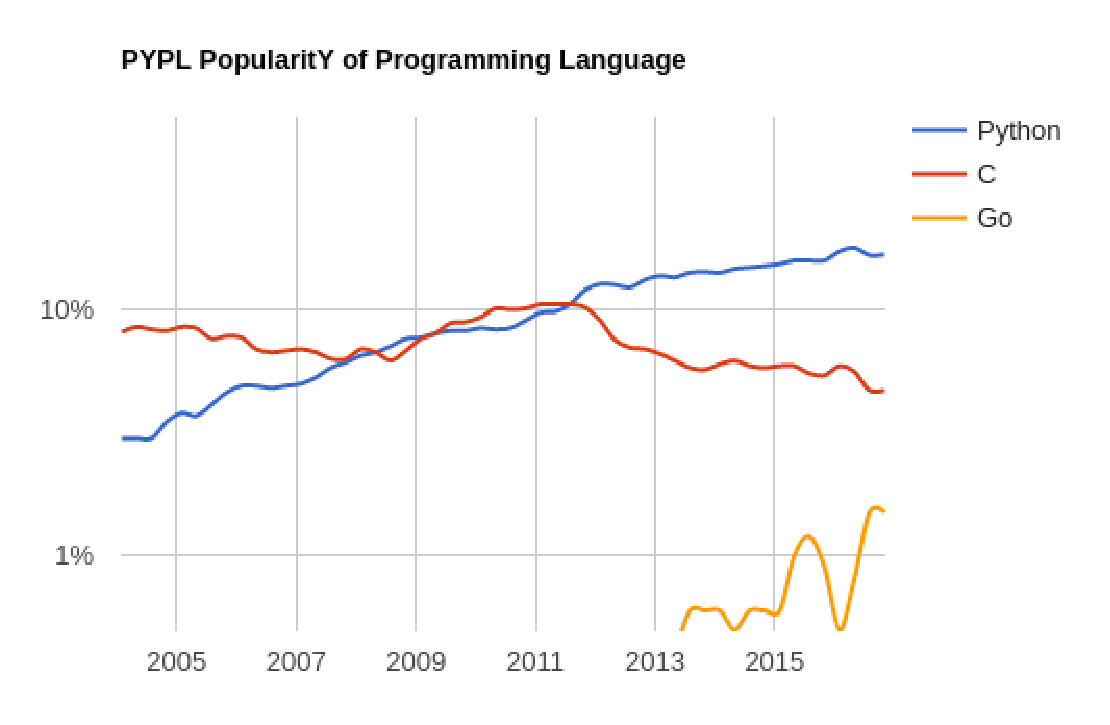
\includegraphics[width=10cm]{pythoncgo.eps}}
		\caption{Python, C, and Go popularity in the US~\cite{PYPL}}
	\end{center}
\end{figure}

\subsubsection{Speed and Space Efficiency}

One benefit of lower-level languages like Go and C is how they treat their
variables. Go and C treat variables differently than some languages such as
Python, which create overhead in order to track type information, and Java,
which converts small ints to Integer class instances when placing them in a
list. An example of this is in the representations of the same value in Go,
Python, and C~\cite{davecheney}:

\begin{lstlisting}
var gocon int32 = 2014              // Go:      4 bytes
uint32_t gocon = 2014;              // C:       4 bytes
gocon = 2014                        #  Python: 24 bytes
\end{lstlisting}

Go performs comparably to C with regard to speed, as well~\cite{benchmarks},
which is considerable since C is often the standard for fast programming
languages. Compared to Python, as would be expected, Go and C can perform up to
45 times faster depending on the workload~\cite{benchmarks}.

\subsubsection{Concurrency}

Concurrency is a key consideration for programming languages when implementing a
software defined network. All operations must happen quickly and in parallel and
must scale effortlessly. Therefore, it is necessary that all operations run in
their own individual threads.

C has an extensive and established framework for parallel computing by utilizing
pthreads. Mutexes can help the programmer protect against race conditions in
their code, but the responsibility is up to the programmer to make their
software thread-safe.

Python has similar tools as C, but the parallelization is handled by a global
interpreter lock (GIL). The GIL is a "mutex that prevents multiple native
threads from executing Python bytecodes at once." GIL is necessary in python
because the underlying C code that implements python is not thread-safe. The GIL
"prevents multithreaded CPython programs from taking full advantage of
multiprocessor systems in certain situations"~\cite{GIL}.

Go, on the other hand, combines the power of C and the ease of use and
lock-handling of Python. You can use goroutines (functions that are capable of
running concurrently with other functions) to create concurrency. Utilization of
goroutines and other builtin language functionalities make concurrency very easy
and lightweight in Go. An example from golang-book.com demonstrates how simple
and lightweight threads in Go can actually be~\cite{goroutines}:

\begin{lstlisting}
package main

import "fmt"

func f(n int) {
	for i := 0; i < 10; i++ {
		fmt.Println(n, ":", i)
	}
}

func main() {
	go f(0)
	var input string
	fmt.Scanln(&input)
}
\end{lstlisting}

\subsubsection{Ease of use}

Python is by far the easiest to learn, use, and read. It focuses on
"readability, coherence, and software quality" and is recognized by many to be
extremely easy to use~\cite{learningpython}.

C, being the oldest and lowest-level language of the three, is not a simple
language to work with. Many things that are normally abstracted away in other
languages are required to be programmed explicitly by the programmer. String
manipulation is especially difficult in C.

Go is easier to learn than C and makes many improvements in terms of ease of
use. It was even designed this way. Go was designed to make programming
efficient in large-scale software development across teams with varying levels
of experience and skill. It was designed with "built-in concurrency and garbage
collection" and includes "rigorous dependency management."~\cite{godesign}.
These features are important for the work required by this project.

Another important note is that the rest of Ciao is written in Go, and while
possible to create interfaces from C or Python for Go, it would be very
difficult. Another option would be to re-implement Ciao in another language,
which is so difficult and time consuming that it cannot even be considered as an
option. With this consideration, Go is the clear winner in terms of ease of use.

\subsection{Direct Comparison}

\begin{center}
	\begin{tabular}{| l | l | l | l | l | l |}
		\hline
		Language & Availability & Efficiency & Concurrency & Ease of use
		\\ \hline
		Go     & 3 & 1 & 1 & 1 \\ \hline
		C      & 1 & 2 & 2 & 3 \\ \hline
		Python & 2 & 3 & 3 & 2 \\ \hline
	\end{tabular}
\end{center}

\subsection{Selection}

Based on the criteria explored above, the Go programming language is the
language we are selecting to implement our solution in. The remainder of the
technical review will be based on the assumption that we will be implementing
our solution in Go.

\section{Logging}

The logging libraries available for Go are almost innumerable, and most are very
similar to each other. It is important that the library is fast, easy to use,
and lightweight. Ciao currently uses the 'glog' standard logging library, but
due to the simplicity of logging it is feasible to choose another option.

\subsection{Options}

\subsubsection{Zap Logger}

Zap is a go logger that advertises "blazing fast, structured, leveled logging in
Go. According to benchmarks against other common logging libraries, Zap is
indeed fast and lightweight in terms of management. There are major concerns
here, however, including the overall size of the package along with its
dependencies and the fact that it is in its beta phase~\cite{zap}.

\subsubsection{Standard 'log' Library}

The log library is standard in Go, and therefore very lightweight with no
external dependencies. It is also simple to use with very many examples
available~\cite{log}. It has less functionality than the zap logger, but we have
very simple requirements.

\subsubsection{Standard 'glog' Library}

The glog library is very similar to the log library but adds a few features,
like an improved leveled-logging functionality~\cite{glog}. The main benefit
here is that glog is used by the rest of the Ciao project, and is therefore
trivial to setup and use in the networking portion~\cite{ciao}.

\subsection{Goals for use in design}

Our goal for the logging module we select is to record important events and
failures for debugging and functional testing.

\subsection{Criteria being evaluated}

\subsubsection{Speed}

As far as speed is concerned, the Zap logger appears to be the fastest of the
options we are exploring, according to benchmarks~\cite{zap}. Glog and log
appear to be very similar, but glog makes a significant efficiency improvement
by binding methods to booleans. This makes it possible to use glog "without
paying the expense of evaluating the arguments to the log"~\cite{glog}.

\subsubsection{Package Size}

It is also important to consider the size of the dependency we are adding to
Ciao. Zap, unfortunately, is a large package that is not already available in
the project.

The log library, being part of the standard library, has no effective size since
it is included with the language dependency.

The glog package, as an external dependency, would normally lose outright in
this category. However, the rest of the Ciao project already uses glog, so
using it in our portion would not add a dependency to Ciao that does not already
exist.

\subsubsection{Ease of Use}

Logging libraries are typically easy to use, and these three options are no
exception. Zap is perhaps the most complicated to setup and use as it requires a
structured log statement~\cite{zap}:

\begin{lstlisting}
logger.Info("Failed to fetch URL.",
	zap.String("url", url),
	zap.Int("attempt", tryNum),
	zap.Duration("backoff", sleepFor),
)
\end{lstlisting}

The standard log library is much simpler. An example of logging a statement in
log~\cite{log}:

\begin{lstlisting}
logger.Print("Hello, log file!")
\end{lstlisting}

The glog library is also very simple, but provides the option of leveled logs.
The following is an example of logging an info and fatal statement, each in a
single line~\cite{glog}:

\begin{lstlisting}
glog.Info("Prepare to repel boarders")
glog.Fatalf("Initialization failed: %s", err)
\end{lstlisting}

\subsection{Direct Comparison}

\begin{center}
	\begin{tabular}{| l | l | l | l |}
		\hline
		Logging library & Speed & Package Size & Ease of Use
		\\ \hline
		log  & 3 & 1 & 2 \\ \hline
		glog & 2 & 2 & 1 \\ \hline
		zap  & 1 & 3 & 3 \\ \hline
	\end{tabular}
\end{center}

\subsection{Selection}

Based on our evaluation of log, glog, and zap, glog comes out on top by a very
small margin. The two simple packages, glog and log, were very close in every
category, and it basically came down to the fact that glog is currently in use
by ciao. We will be using glog for logging events in our portion of the project.

\section{Functional Testing Frameworks}

There are several testing frameworks available for Go. These range from the
basic and simple 'testing' library to the more complicated and in-depth GoConvey
and Ginkgo frameworks. Depending on our choice here, we could either add too
much extraneous work getting a testing framework setup, or we could end up with
simple tests that do not meet our needs.

\subsection{Options}

\subsubsection{Standard 'testing' library}

The simplest and most lightweight option is the standard 'testing' library. This
can be expanded with the additional 'testify' library, which adds functionality
for mocking, assertions, HTTP protocol, and basic functions.

\subsubsection{GoConvey}

GoConvey is a testing framework that allows you to track your test status with a
generated web UI. The tests can run automatically every time you save a .go
file. GoConvey also generates an html test coverage report that allows you to
review where your tests are falling short.

\subsubsection{Ginkgo}

GinkGo is a testing framework that allows you to write specifications for your
tests. It is lighter-weight than GoConvey and works primarily from the command
line. GinkGo takes a black box approach to testing.

\subsection{Goals for use in design}

The goal of the testing framework is to continuously verify our solution.
Testing is important for any software, but it is particularly important in cloud
orchestration networking. Our solution must be robust, and that can only be
verified through rigorous testing.

\subsection{Criteria being evaluated}

The two important criteria when selecting a testing framework is the
capabilities of the framework itself and the complexity of the framework. On one
hand we want the tests to be powerful and support important features such as
mocking and assertion. On the other hand we do not want the test framework to be
so complicated that it is difficult to write tests.

\subsubsection{Capability}

The most important aspect of the testing framework is its ability to perform
mocking. This is essential in unit testing. All three of the test frameworks
allow the programmer to perform mocking.

Another important capability is assertion testing. Once again, all three support
assertion tests.

A third important capability is randomization in testing. This is the best way
to ensure corner cases are hit. This aspect, however, is provided by the Go
standard library and therefore does not factor into this analysis.

One area where GoConvey shines is in its ability to perform testing analysis and
output an easy-to-use web user interface. Ginkgo also provides some extra
functionality related to black box testing.

\subsubsection{Complexity}

Of the three frameworks, the testing package is by far the simplest. Since it
exists in the standard library, there is no overhead of installation or setup to
get started writing tests~\cite{testing}.

Ginkgo is slightly more complicated to setup, since it is necessary to install
and run a few Ginkgo-specific commands before ready to start writing tests. Once
everything is ready, you can write tests, but must use Ginkgo-specific keywords
and tests to utilize its full potential~\cite{ginkgo}.

The most complex framework is the GoConvey suite. This is no surprise,
considering how powerful it is. GoConvey requires the programmer to view the
test results in a browser, as well~\cite{goconvey}. This is difficult for our
purposes, since we will be doing much of our development on remote machines via
ssh, and will not have access to an X server to view the results.

\subsection{Direct Comparison}

\begin{center}
	\begin{tabular}{| l | l | l |}
		\hline
		Framework & Capability & Complexity
		\\ \hline
		testing  & 3 & 1  \\ \hline
		GinkGo   & 2 & 2  \\ \hline
		GoConvey & 1 & 3  \\ \hline
	\end{tabular}
\end{center}

\subsection{Selection}
Although the direct comparison reveals that all three are equally averaged to
second place overall, the decision here is weighted towards the lowest in
complexity. Our solution will be complex and difficult to implement, we do not
want to have to worry about learning how to use a complicate testing framework
on top of everything else. The standard 'testing' package will be used for
functional and unit testing of our solution.

% Cody
\section{Packet Level Protocols}
One of the main components of our system is deciding which protocol will be
used to move data from one node to the next. Ciao provides its own data
transfer protocol using SSNTP. Comparing how SSNTP works in general to other
data transfer formats will provide insight into which protocol should be used.

\subsection{Options}

\subsubsection{SSNTP}
Simple and Secure Node Transfer Protocol is Intel's solution for the transfer
of data inside of Ciao networks. It is based on Transport Layer Security (TLS),
the defacto standard for secure data transfer over the Internet. Part of what
sets Ciao apart from the competition is its simplicity, as well as concise
message format~\cite{ssntp}.

\subsubsection{TLS}
Transport Layer Security, or TLS, is the contemporary standard for secure data
transfer across the Internet. It was built as an improvement upon the Secure
Socket Layer protocol. It has great appeal as it is widely utilized, modern,
and well studied~\cite{tls}.

\subsubsection{SSL}
Secure Socket Layer, or SSL, was the first version of what eventually became
TLS following its third major revision. Originally utilized in Netscape, it
wasn't widely utilized until it's third major revision. Secure Socket Layer
encrypts at the application layer, allowing broad general use. While being
somewhat older than the other protocols on the list, it is well understood and
the security has been well proven~\cite{ssl}.

\subsection{Goals for use in design}
The primary goal of the selected protocol is fast, stable, secure, and
scalable communication between compute nodes and the orchestration node in
Ciao. These are simple, but critical goals for the project.

\subsection{Criteria being evaluated}
The criteria for each protocol will be their security capabilities, protocol
overhead, and ease of use. While stability is a concern, each protocol has
shown stability through implementation in other applications many times over.
This will be less of a focus for evaluation purposes.

\subsubsection{Speed}
Speed is a major consideration when working with a software defined network.
Our final selection for a protocol needs to be fast. Any major delays in
communication due to encryption or protocol overhead is a concern. While each
implementation of the protocol will have its pros and cons, here the focus
will be on application overhead to keep the metric in measurable territory.

SSL has two major components, the message protocol, and the handshake protocol. The
handshake protocol is important as it ensures the overall security and
authenticity of the communication between point A and point B
~\cite{topdown-ssl}.

%Diagram of SSL handshake here
\begin{figure}[H]
	\begin{center}
		\makebox[\textwidth]{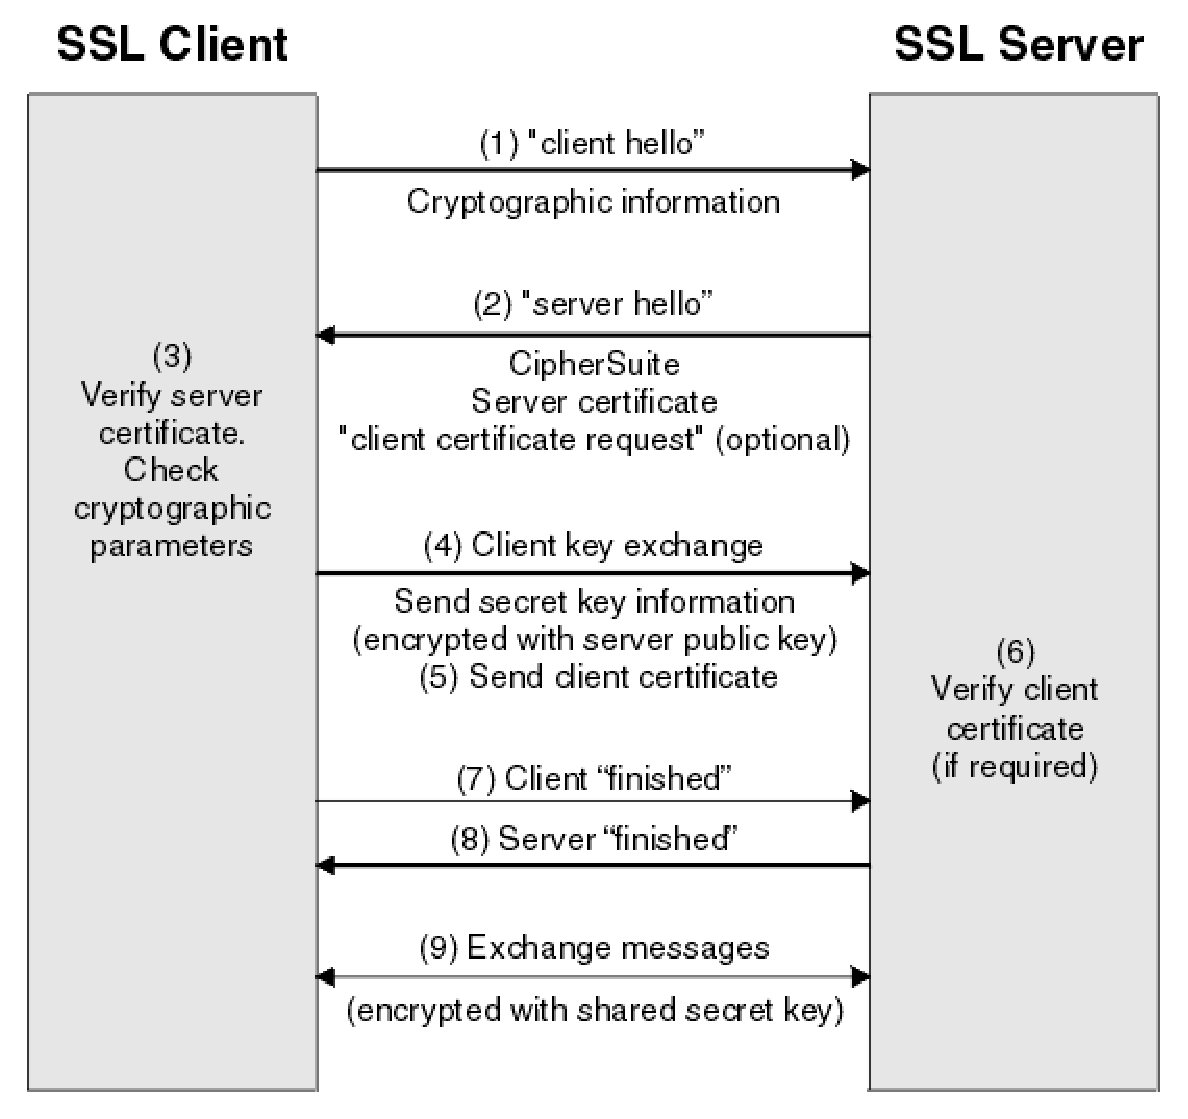
\includegraphics[scale=.35]{ssl-diag.eps}}
		\caption{Simple SSL and TLS Handshake\cite{ibm-diagram}}
	\end{center}
\end{figure}

The SSL/TLS handshakes are identical. As far as overhead the two protocols
are very similar. The primary difference between them is their security levels,
which will be discussed in the following section.

The SSNTP equivalent of a handshake is called a SSNTP Connection. There is a
fundamental difference that needs to be noted between SSNTP and the other two
options. The difference is that the computers running SSNTP client software
only have to do an authentication handshake, or SNTP Connection in this case,
once. Once the client knows which server it is talking to, all connections
no longer require a handshake step. This is a massive drop in needed overhead.
\cite{ssntp}. Once the handshake is established, the client communicates with
the server in an asynchronous fashion as needed.

\subsubsection{Security}
Security is important in choosing a communication protocol. If it wasn't, we
could just use TCP, the protocol that all of these security protocols
encapsulate.

SSL is unfortunately at the bottom of the list as far as the
protocols listed here are concerned. Has a few vulnerabilities that have been
found in the decade or so. While some of these are less of an issue, one attack
in particular called POODLE has caused several major groups to call for SSL 3.0
to be deprecated~\cite{poodle}. While calling into question consideration for
using this protocol on this system, it is still better than not having any
security or encryption at all.

TLS is much better on this front as it is continually being updated. The latest
release, version 1.2, uses AES, RC4, and a few other modern encryption ciphers~
~\cite{tls}. Which encryption cipher is used is negotiated between the host and
the client before communication begins.

SSNTP uses the TLS encryption protocols. On this front, it is equal to TLS.

\subsubsection{Accessibility}
All of the above protocols are well documented and easy to implement. In the
scope of the project, however, SSNTP would be easier to use because other
components of the system already use it. For that reason alone, it is simpler
to get working for the project.

\subsection{Direct Comparison}
\begin{center}
	\begin{tabular}{| l | l | l | l |}
		\hline
		Protocol & Speed & Security & Accessibility \\ \hline
		SSNTP & 1 & 1 & 1 \\ \hline
		SSL & 2 & 3 & 2 \\ \hline
		TLS & 2 & 1 & 2 \\ \hline
	\end{tabular}
\end{center}

\subsection{Selection}
For our project, the technology for protocols will be SSNTP. It does what SSL
and TLS do equally security wise, but is much more light weight and is more
accessible in the context of the project.

%----------------------

\section{Network Virtualization}
Because Ciao works off of a virtual network, it's important to pick the right
tool for encapsulating packets to ensure they arrive at their destination. The
standard virtual network tools have proven to be limited in their ability to
scale. What the following tools do is allow for networks to scale to order of
magnitudes higher than a standard virtual network would. As for virtual networks, 
virtual networks allow for virtual machines, or containers (docker, rkt) to be
visible to the virtual network switch. This is powerful as a VM or container
does not have a physical network card.

As we move to Open vSwitch, it gives us the option of using Network
Virtualization using Generic Routing Encapsulation (nvGRE) or Virtual Extensible
Local Area Network (VxLAN). Along with these two, a third option, Stateless
Transport Tunneling (STT), will be contrasted to see which option fits the
project needs best.

\subsection{Options}
\subsubsection{VxLAN}
VxLAN is a relatively new virtualization standard developed by a few major
players in the network industry. Cisco, VMware, Citrix, and Redhat all came
together to work on this standard to resolve the major problem of massive
virtual networks. VxLAN's primary advantage is that it has a massive address
space, about sixteen million, and that it's overall overhead increase is only
fifty bytes~\cite{vxlan}. Speed will be a deciding factor in which interface
is chosen, so a fifty byte overhead is quite good.

\subsubsection{nvGRE}
NvGRE is another relatively new virtualization standard developed in tandem by
Microsoft, HP, Intel, HP, and Dell~\cite{nvgre-info}. NvGRE sports a few of the
same features as VxLAN, the primary difference between the two being the header
field. They use different UDP port numbers and use a different bit to indicate
that encapsulation has occurred~\cite{nvgre}. The primary difference between the
two is going to be overall performance in our network setup.

\subsubsection{STT}
Stateless Transport Tunneling is a protocol developed by VMware to handle the
same problem stated by the above protocols, but is primarily used to communicate
between virtual switches. It is quite different than the other protocols as it
carries much larger packets, up to sixty-four kilobytes, and it's overhead in
general is much larger. This could be a major problem when it comes to choosing
a protocol to use as overhead must be minimized.

\subsection{Goals for use in design}
The goal for these technologies is minimization of overhead while allowing for a
virtual network to be mapped and allow for thousands of VMs and containers to
become available easily. This problem of scalability is a major one, and one
that has to be addressed when created large networks of computers hosting VMs or
virtual machines.

\subsection{Criteria being evaluated}
The primary attribute being evaluated here is performance or lack of overhead.
Performance and overhead go hand in hand, so they will be the primary metric of
evaluation for this project. In terms of speed, all of these protocols move at
the speed of hardware, so overhead makes sense for evaluation of the speed of
the protocol. Less overhead equals more packets moved per second.

\subsubsection{Overhead}
NvGRE and VxLAN share almost identical header formats, with the primary
difference in how they encapsulate their packets. NvGRE uses existing tunneling
functionality in a TCP packet to encapsulate the data. All that is different is
that is alters the twenty-four bits of data usually used for regular GRE to
identify itself. This quite useful as it allows a great deal of existing
hardware to support this "new" protocol. The primary downside here being that
loadbalancers and firewalls have to expand the the full packet, removing GRE, to
inspect the packet. This could be a major slowdown if the packet inspection is a
frequent activity~\cite{nvgre-vs-vxlan}.

VxLAN on the otherhand, while adding an additional fifty bytes of overhead to
every packet, still requires the reversal of the encapsulation of every packet
out of the VxLAN format. The other downside here being reduced compatibility
with existing routing hardware. This is less of an issue for this project as all
of our routing devices will be implemented in software~\cite{nvgre-vs-vxlan}.

STT has a significant disadvantage in the area of overhead when it comes to
general use. It's primary design purpose at VMware was to carry large amounts of
data from point A to point B. In our use case, it doesn't make much sense. Its
overall packet header size will be between sixty-two bytes to eighty bytes. This
is much larger than the other two. While this may not be a huge issue for VM to
VM traffic, it becomes an issue when it travels across physical networks
~\cite{stt}.

\subsection{Direct Comparison}
\begin{center}
	\begin{tabular}{| l | l |}
		\hline
		Protocol & Overhead \\ \hline
		nvGRE & 1 \\ \hline
		VxLAN & 2 \\ \hline
		STT & 3 \\ \hline
	\end{tabular}
\end{center}

\subsection{Selection}
For the purposes of the project, we will work with nvGRE in order to provide the
lowest overhead. Live testing of nvGRE and VxLAN are part of the project. While
it is difficult to tell during the design phase which will be better in
production, on paper nvGRE seems to work better for our needs.

%----------------------

\section{Network Bridge Implementation}
Part of the project is generating GRE tunnels. Tunnels are very important when
dealing with virtual networks. It allows a given VM to be mapped to the same
network that another VM is on. This allows an arbitrary network to be created
where a given set of VMs can be treated as a single network, regardless of their
actual physical location. This allows a tenant to rent a set of VMs regardless
of the set of servers they are on. While the GRE tunnels themselves are often
identical, which is often the case when a standard exists, the features of the
individual interfaces vary. There are two main options for this particular
technology: Linux Bridges and Open vSwitch bridges. The third alternative, is
not using them.

\subsection{Options}

\subsubsection{Linux Bridges}
Linux bridges are the standard for any user to create a network bridge from
one network location to another. Linux bridges, as the name implies, ships with
the Linux kernel. The big attraction to Linux bridges is that they are tried and
tested, as well as being relatively simple. While being great for consistent
deployment across devices, there are no updates occurring in the development
area outside of the occasional security patch~\cite{ovs-linuxbridge}.

\subsubsection{Open vSwitch Bridge}
Open vSwitch is the only current area of major network innovation in the area of
network bridging on Linux. While functionally, Linux bridges and OVS bridges are
the same, OVS supports packet acceleration frameworks that Linux bridges do not
~\cite{ovs-linuxbridge}.

\subsubsection{No Bridge}
The alternative to these two technologies is not having a bridge, and manually
having to bridge networks with physical cabling. While possible, this is not a
cost-effective method nor one that is easily accomplished without great
manpower.

\subsection{Goals for use in design}
The goal in design of this system is to add an interface with the possibility
for future expansion of capabilities as new systems and algorithms are created
to improve bridging. For this implementation, larger feature sets, and an
actively updated code base are ideal.

\subsection{Criteria being evaluated}
For this component, available features, as well as an actively updated code base
are needed. This component is a preliminary for future implementation
improvements, more concisely, it is groundwork.

\subsubsection{Feature Set}
In this metric, OVS vastly outstrips Linux bridges, and both Linux bridges and
OVS are better than nothing at all. OVS has an actively updated code base, and
has many more features available than Linux bridges~\cite{ovs-linuxbridge}. One
of the main features that make OVS bridges more appealing than Linux bridges are
the availablilty of package acceleration frameworks. Not having any bridge at
all, on the other hand, falls outside of our project requirements, and therefore
is not a good option.

\subsection{Direct Comparison}
\begin{center}
	\begin{tabular}{| l | l |}
		\hline
		Bridge & Features \\ \hline
		Linux Bridge & 2 \\ \hline
		OVS Bridge & 1 \\ \hline
		None & 3 \\ \hline
	\end{tabular}
\end{center}

\subsection{Selection}
OVS is the right choice for this project, and the goals Intel has in the future
for Ciao. It opens open a large feature set to be utilized, as well as opens
Ciao up to benefit from any innovations made in OVS in the future.

%-----------------------------------------------

%Software switches for CNCI and CNs
\section{Software Switch for the Compute Node Concentrator and Compute Nodes}
As part of creating a software defined network we need a software switch for the compute node concentrator(CNCI) and compute nodes(CN). 
Intel suggested we use Open vSwitch as part of the project requirements. 
The software switch needs to run on all of the platforms the Ciao supports, support GRE tunnels, VxLAN/nvGRE, and DPDK.
I did some research on software switches and came up with LINCX and Lagopus as possible alternatives.

\subsection{Options}
\subsubsection{Open vSwitch}
Open vSwitch is an open source software switch written in platform independent C~\cite{ovs-readme}.
This means that it will run on all of the platforms supported by Ciao.
It can operate as a kernel module paired with a daemon, or as user space application.
For our use case we are interested in the kernel module paired with the daemon.
Open vSwitch can be configured using a remote configuration server which works well with the CNCI and CN model.
It has support for GRE tunnels, VxLan, nvGRE, and DPDK.

\subsubsection{LINCX}
LINCX is an open source software switch written in Erlang~\cite{lincx}.
It requires the Erlang runtime be installed on the system it is running on.
This means it should run on the platforms Ciao supports, but it adds another dependency.
LINCX gets its configuration from a local configuration file.
It does not have documented support for DPDK, or GRE tunnels.

\subsubsection{Lagopus}
Lagopus is an open source software switch written in C~\cite{lagopus}.
It only runs on Intel x86 machines.
The only operating systems it officially supports are Ubuntu 14.04, Ubuntu 16.04, CentOS 7, FreeBSD, and NetBSD.
It has support for DPDK, GRE tunnels, and VxLAN.


\subsection{Software switch comparison}

\begin{center}
	\begin{tabular}{| l | l | l | l | l | l |}
		\hline
		Name & GRE & VxLAN & Remote configuration & Language & DPDK support  \\ \hline
		Open vSwitch & Yes & Yes & Yes & C & Yes \\ \hline
		LINCX & No & Yes & No & Erlang & No \\ \hline
		Lagopus & Yes & Yes & Yes & C & Yes \\ \hline
	\end{tabular}
\end{center}

\subsection{Selection}
We selected Open vSwitch for use as our software switch. 
This is the option that Intel wants us to use, and after researching other switches I agree with their choice.
It has support for a wide variety of platforms unlike Lagopus which only officially supports Ubunutu 14.04 and Ubuntu 16.04, CentOS 7, NetBSD, and FreeBSD.
LINCX supports any platform Erlang runs on, but does not have documented support for DPDK.
In addition to the platform requirements, Open vSwich allows for configuration to be provided by a server.
Both LINCX and Lagopus only support configuration via local configuration files.
I could not find documented support for creating GRE tunnels with LINCX which removes it from the consideration.
Combined with its lack of DPDK support it is not a good selection for this project.
Lagopus has support for DPDK, as well as GRE tunnels and VxLAN, but it does not officially support all of the platforms we need it to. 
It also lacks the remote configuration support that Open vSwitch has.
After taking all of this into consideration Open vSwitch is the best choice.


\section{Network Latency Measurement Tools}
One of our project requirements is to conduct network performance testing on our implementation.
The purpose of testing network performance is to determine which tunneling protocols to use, 
and how our Open vSwitch implementation compares to the initial implementation.
One of the metrics we are using to determine network performance is latency.
Latency is how long it takes data to travel between hosts on a network~\cite{topdown-ssl}.

\subsection{Tool Requirements}
The tool must work on Clear Linux which is the Linux distribution we are running Ciao on.
It must allow us to measure network latency. 
It must have a command line interface.
We must be able to capture the output and easily translate it into useful data. 
We should be able to graph the results. 

\subsection{Options}
\subsubsection{Wireshark}
Wireshark is a network protocol analyzer that can be used to measure many network statistics including latency and throughput~\cite{wireshark}. 
It has a command line interface called tshark.
It supports saving network traffic to a capture file that can be analyzed at a later date.
Wireshark only analyzes network traffic, it does not generate it.
We would need to use Wireshark in combination with one of their recommended traffic generator tools to calculate latency~\cite{wireshark-tools}.
Wireshark is very complex and has a lot of features we do not require for our use case.
If we take the capture file it generates and open it with the GUI version of Wireshark we can generate graphs without feeding the data into another application.

\subsubsection{Ping}
Ping is a command line tool that can be used to measure the latency between two hosts~\cite{ping}.
It is a standard networking tool that is well tested and simple to use.
The output is human readable, but not very machine readable. 
We would need to parse the output into a more computer friendly format before graphing it.
It does not support throughput statistics so we would need to use another tool to calculate throughput.
It can be configured to send a specific number of packets and will return the latency for each packet sent, as well as the minimum, average and maximum latency for the packets sent.
\begin{lstlisting}[caption = Example ping usage, basicstyle=\ttfamily]
[smithgar@flip3:~ ] > ping -c 5 oregonstate.edu
PING oregonstate.edu (54.244.95.93) 56(84) bytes of data.
64 bytes from ec2-54-244-95-93.us-west-2.compute.amazonaws.com (54.244.95.93): icmp_seq=1 ttl=42 time=10.6 ms
64 bytes from ec2-54-244-95-93.us-west-2.compute.amazonaws.com (54.244.95.93): icmp_seq=2 ttl=42 time=10.6 ms
64 bytes from ec2-54-244-95-93.us-west-2.compute.amazonaws.com (54.244.95.93): icmp_seq=3 ttl=42 time=12.8 ms
64 bytes from ec2-54-244-95-93.us-west-2.compute.amazonaws.com (54.244.95.93): icmp_seq=4 ttl=42 time=10.6 ms
64 bytes from ec2-54-244-95-93.us-west-2.compute.amazonaws.com (54.244.95.93): icmp_seq=5 ttl=42 time=11.1 ms

--- oregonstate.edu ping statistics ---
5 packets transmitted, 5 received, 0\% packet loss, time 4005ms
rtt min/avg/max/mdev = 10.628/11.204/12.877/0.871 ms
\end{lstlisting}

\subsubsection{Qperf}
Qperf is a command line tool that can be used to measure network latency for both TCP and UDP packets~\cite{qperf}.
It must be run in a client/server configuration.
The client can then make requests to the server and receive latency statistics.
The output is in human readable format.
The following is an example taken from OpsDash showing how to use qperf to measure UDP bandwidth and latency~\cite{qperf-example}.
\begin{lstlisting}[caption = Using qperf to measure UDP latency,basicstyle=\ttfamily]
root@node2:~> qperf -v 10.99.0.1 udp_lat
udp_lat:
    latency        =  46.7 us
    msg_rate       =  21.4 K/sec
    loc_cpus_used  =  11.5 % cpus
    rem_cpus_used  =    10 % cpus
\end{lstlisting}


\subsection{Network Latency Tool Comparison}

\begin{center}
	\begin{tabular}{| l | l | l | l | l |}
		\hline
		Name & Output type & Single tool & TCP & UDP \\ \hline
		Wireshark & Capture File & No, requires multiple tools & Yes & Yes \\ \hline
		Ping & Human readable text & Yes & Yes & No \\ \hline
		Qperf & Human readable text & Yes & Yes & Yes \\ \hline
	\end{tabular}
\end{center}

\subsection{Selection}
I chose qperf as the tool for latency measurement.
Wireshark requires more setup and configuration than qperf.
Ping does not allow us to check the latency of UDP connections.
We will need to install qperf on each of the machines we are performing network tests on by building it from source.
I tested the installation process in a Docker container and it only takes a couple of minutes to download and build the source.

\section{Network Throughput Measurement Tools}
As part of the network performance testing we are measuring network throughput.
Throughput is how much data can be transferred between two hosts on a network in a fixed amount of time~\cite{topdown-ssl}.

\subsection{Tool Requirements}
The tool must work on Clear Linux which is the Linux distribution we are running Ciao on.
It must allow us to measure network throughput for both TCP and UDP packets. 
It must have a command line interface.
We must be able to capture the output and easily translate it into useful data. 
We should be able to graph the results. 

\subsection{Options}

\subsubsection{iPerf3}
iPerf3 is an open source tool for measuring network throughput~\cite{iperf}.
It runs in a client server configuration on two hosts and measures throughput between the client and server.
It can be configured to use random data, or to send a file across the network.
It supports both TCP and UDP, as well as IPv4 and IPv6.
It can be bound to specific network inferfaces on devices with more than one network interface.
It can be configured to produce output in JSON format. 
This is an advantage because it is human readable, and easily parsible with many programming languages.
Below is an example from the iPerf3 documentation of running it from the command line to measure the latency between hosts~\cite{iperf}.
\begin{lstlisting}[caption = Sample iPerf 3 usage, basicstyle=\ttfamily]
node2> iperf -s
------------------------------------------------------------
Server listening on TCP port 5001
TCP window size: 60.0 KByte (default)
------------------------------------------------------------
[  4] local <IP Addr node2> port 5001 connected with <IP Addr node1> port 2357
[ ID] Interval       Transfer     Bandwidth
[  4]  0.0-10.1 sec   6.5 MBytes   5.2 Mbits/sec

node1> iperf -c node2
------------------------------------------------------------
Client connecting to node1, TCP port 5001
TCP window size: 59.9 KByte (default)
------------------------------------------------------------
[  3] local <IP Addr node1> port 2357 connected with <IP Addr node2> port 5001
[ ID] Interval       Transfer     Bandwidth
[  3]  0.0-10.0 sec   6.5 MBytes   5.2 Mbits/sec
\end{lstlisting}


\subsubsection{Wireshark}
Wireshark is a network protocol analyzer that can be used to measure many network statistics including latency and throughput~\cite{wireshark}. 
It has a command line interface called tshark.
It supports saving network traffic to a capture file that can be analyzed at a later date.
Wireshark only analyzes network traffic, it does not generate it.
We would need to use Wireshark in combination with one of their recommended traffic generator tools to gather network throughput metrics~\cite{wireshark-tools}.
Wireshark is very complex and has a lot of features we do not require for our use case.
If we take the capture file it generates and open it with the GUI version of Wireshark we can generate graphs without feeding the data into another application.

\subsubsection{Netcat}
Netcat is a tool that can be used to read and write data across networks from the command line~\cite{netcat}.
When combined with timing software it can be used to calculate throughput.
It is a standard networking utility and is well tested.
The downsides to using Netcat are that you have to generate input using a tool such as dd.
\begin{lstlisting}[caption = Caclulating throughput with netcat and dd~\cite{nc-example}, basicstyle=\ttfamily]
server\$: nc -v -l 2222 > /dev/null
client\$: dd if=/dev/zero bs=1024K count=512 | nc -v \$IP_OF_SERVER 2222
Result from dd:
536870912 bytes (537 MB) copied, 4.87526 s, 117 MB/s
\end{lstlisting}


\subsection{Network Throughput Tool Comparison}

\begin{center}
	\begin{tabular}{| l | l | l | l | l |}
		\hline
		Name & Output type & Single Tool & TCP & UDP \\ \hline
		iPerf3 & Human readable text or JSON & Yes & Yes & Yes \\ \hline
		Wireshark & Capture File & No, requires additional tools & Yes & Yes \\ \hline
                Netcat & Human readable text & No, requires additional tools & Yes & Yes \\ \hline
	\end{tabular}
\end{center}

\subsection{Selection}
I chose iPerf3 as the tool for gathering network throughput statistics because it handles measuring throughput without any special configuration or other tools, and allows us to output the data in human readable format or JSON.
This makes it easy to graph and analyze the results.
Wireshark offers many of the same features as iPerf3 but it requires more set up and configuration, and does not output its results in as universal of a format. 
While Wireshark's built in graphing feature is useful, it does not outweigh the downsides.
We would also need to use one of the recommended tools to generate network traffic~\cite{wireshark-tools}.
Netcat must be used in combination with other utilities such as dd and does not output its results in as nice of a format as iPerf3.

\section{Conclusion}
We explored nine components of our system and three technologies of each,
resulting in an overview and comparison of twenty-seven technologies. We settled
on one or more technologies per comparison. A summary of the selected
technologies are listed below.

\begin{enumerate}
	\item Programming Language - Golang
	\item Logging Library - glog library
	\item Functional Testing Framework - logging library
	\item Packet Level Protocols - SSNTP
	\item Switch Implementation - nvGRE
	\item Bridge Implementation - Open vSwitch Bridge
	\item Software Switch for CNCI and CNs - Open vSwitch
	\item Network Latency Measurement Tool - Qperf
	\item Network Throughput Measurement Tool - iPerf3
\end{enumerate}

These selections were made based on research, and not trial implementation.
These selections may change if blocking issues are discovered in the future.
\section{References}

\bibliographystyle{IEEEtran}
\bibliography{tech}

\end{document}
